Die technischen Mängel der Hochdruckdampfmaschinen waren einer der Gründe, warum sich Robert Stirling mit der Entwicklung einer damals neuartigen Wärmekraftmaschine beschäftigte. Im Jahr 1816 meldete Stirling den nach ihm benannten \textit{Stirlingmotor} bzw. Heißluftmotor zum Patent an. In Versuch 222 werden wir uns anhand eines Modells mit der Funktionsweise und verschiedenen Anwendungen des Stirlingmotors genauer auseinandersetzen.

\subsection{Physikalische Grundlagen}

Grundsätzlich lässt sich zwischen zwei verschiedenen Typen von Heißluftmotoren unterscheiden, dem $\gamma$-Typ und dem $\beta$-Typ Heißluftmotor. Die Funktionsweise beider Typen basiert auf den gleichen Prinzipien, während beim $\gamma$-Typ der Prozess jedoch auf zwei Verbunde separate Zylinder aufgeteilt ist, kommt der $\beta$-Typ mit einem Zylinder aus. Da wir im Versuch alle Experimente ausschließlich an einem $\beta$-Typ Heißluftmotor durchführen, wird sich die folgende Einleitung auch auf diesen beschränken.

\begin{figure}[H]
  \centering
  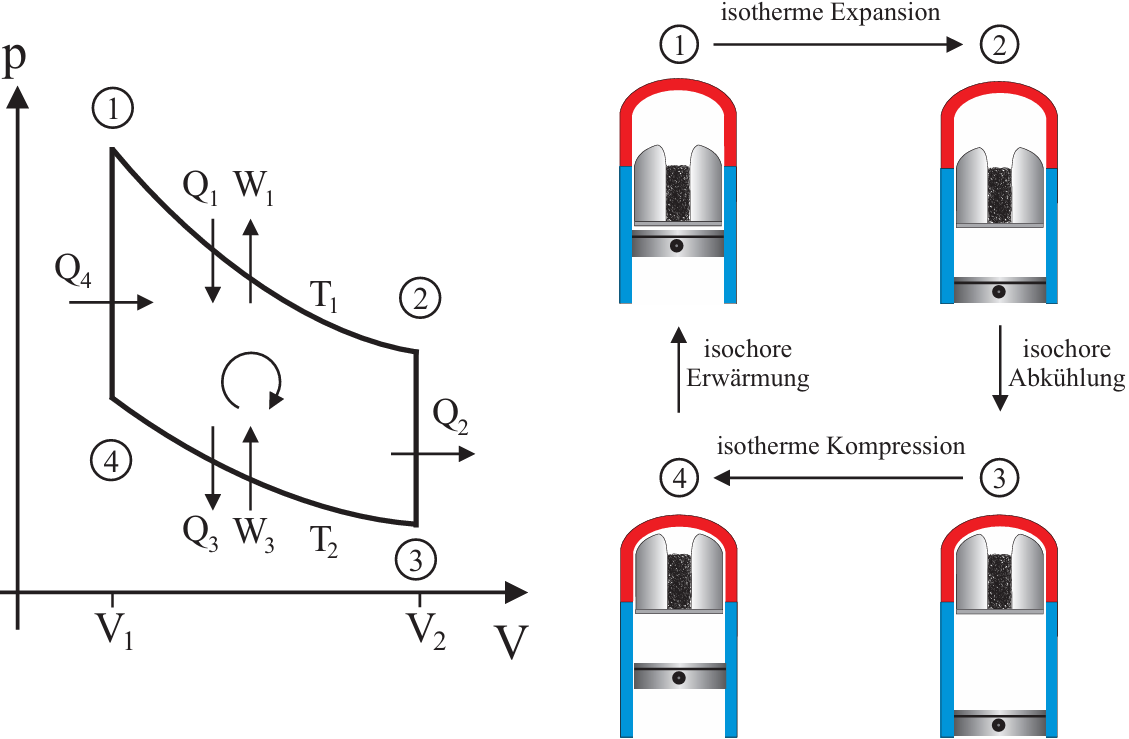
\includegraphics[width=.65\textwidth]{files/type_b_pv_scheme.png}
  \caption{pV-Diagramm der Funktionsweise und schematische Darstellung der Kolbenbewegung des $\beta$-Typ Heißluftmotors}
  \label{fig:type_b_pv_scheme}
\end{figure}

Wie \abbref{fig:type_b_pv_scheme}, rechts, zu entnehmen bewegen sich im Zylinder des $\beta$-Typ Heißluftmotors zwei Kolben, der Arbeitskolben und der Verdrängerkolben. Der Verdrängerkolben dient dazu, das Gas im Zylinder zwischen dem oberen beheizten und dem unteren gekühlten Teil hin und her zu schieben. Der Arbeitskolben ist für die Kompression und Expansion des Gases im Zylinder zuständig. Das $pV$-Diagramm, in \abbref{fig:type_b_pv_scheme}, links, zeigt eine idealisierte Darstellung der thermodynamischen Zustandsänderungen, den \textit{Stirling-Prozess}, welche durch die Kolbenbewegung erzielt wird.

Zur genaueren Beschreibung des Prozesses betrachten wir die durch den ersten Hauptsatz der Thermodynamik gegebene Gleichung
\begin{align}
  \dd{Q} = \dd{U} + p\dd{V},
\end{align}
welchen wir unter der Annahme eines idealen Gases umschreiben können zu
\begin{align}
  \dd{Q} = C_V \nu \dd{T} + p\dd{V}.
\end{align}
Über die molare Wärmekapazität $C_V$ und die Gasmenge $\nu$ in $\si{\mol}$ lässt sich die direkte Auswirkung auf die Temperatur durch Änderung der inneren Energie formulieren.

Mit dieser Gleichung lassen sich die Energiebilanzen der vier Zustandsänderungen in \abbref{fig:type_b_pv_scheme} aufstellen.

\textbf{Zustand 1 \textrightarrow{} 2} läuft durch eine isotherme Expansion ab. Die Luft im heißen Zylinderbereich wird aufgeheizt und nimmt dabei die Wärmemenge $Q_1$ auf. Sie dehnt sich folglich aus und verrichtet dabei die Arbeit $W_1$ durch die Verschiebung des Arbeitskolbens. Es gilt
\begin{align}
  \dd{Q_1} = p \dd{V} = \nu R T_1 \frac{\dd{V}}{V},
\end{align}
wobei wir in der letzten Gleichheit auf das ideale Gasgesetz zurückgreifen. Durch Integration vom Volumen $V_1$ zu $V_2$ erhalten wir einen Ausdruck für die Wärmemenge $Q_1$, welche zugleich der vollständigen Volumenarbeit $W_1$ entspricht.
\begin{align}
  Q_1 = \nu R T_1 \ln\frac{V_2}{V_1} = W_1
\end{align}

\textbf{Zustand 2 \textrightarrow{} 3} ist eine isochore Abkühlung des Gases von der Temperatur $T_1$ auf die Temperatur $T_2$. Diese wird dadurch hervorgerufen, dass der Verdrängerkolben die heiße Luft in den gekühlten Bereich des Zylinders verschiebt. Bei einer isochoren Zustandsänderung bleibt das Volumen gleich, es gilt also
\begin{align}
  \dd{Q_2} = C_V \nu \dd{T}.
\end{align}
Durch Integration erhalten wir den Ausdruck
\begin{align}
  Q_2 = - C_V \nu (T_1 - T_2)
\end{align}
für die nach außen über das Kühlsystem abgeführte Wärmemenge. In diesem Arbeitstakt wird keine mechanische Arbeit verrichtet, es gilt also $W_2 = 0$.

Bei der isothermen Kompression in \textbf{Zustand 3 \textrightarrow{} 4} komprimiert der Arbeitskolben bei seiner Bewegung nach oben die kalte Luft. Dabei verrichtet dieser am Gas die Volumenarbeit
\begin{align}
  W_3 = -\nu R T_2 \ln\frac{V_2}{V_1},
\end{align}
welche gleich der Wärmemenge $Q_3$ ist, die über das Kühlsystem abgeführt wird. Mathematisch folgen wir hier denselben Überlegungen wie beim Übergang 1 \textrightarrow{} 2.

Der Übergang \textbf{Zustand 4 \textrightarrow{} 1} läuft erneut isochor ab. Hierbei wird das Gas durch die Bewegung des Verdrängerkolbens nach oben in den heißen Zylinderbereich geschoben. Die Wärmemenge, welche das Gas hier aufnimmt, ist Analog zur Zustandsänderung 2 \textrightarrow{} 3 gegeben durch
\begin{align}
  Q_4 = C_V \nu (T_1 - T_2).
\end{align}
Auch hierbei wird keine mechanische Arbeit verrichtet, es gilt somit erneut $W_4 = 0$.

Die gesamte geleistete Nutzarbeit $W_N$ erhalten wir aus dem Kurvenintegral über den gesamten Kreisprozess, welches sich auf die Summe
\begin{align}
  W_N = W_1 + W_3 = \nu R(T_1 - T_2) \ln\frac{V_2}{V_1}
\end{align}
reduziert. Aus dem Verhältnis zwischen der Nutzarbeit und der aufgenommenen Wärmemenge $Q^+$ ergibt sich der ideale thermische Wirkungsgrad nach
\begin{align}
  \eta_{th} = \frac{W_N}{Q^+}. \label{eq:eta_th}
\end{align}

Für die aufgenommene Wärmemenge $Q^+$ gilt zunächst
\begin{align}
  Q^+ = Q_1 + Q_4 = \nu R T_1 \ln\frac{V_2}{V_1} + C_v \nu (T_1 - T_2).
\end{align}
Dies liegt daran, dass die in Takt 2 \textrightarrow{} 3 an das Kühlsystem abgegebene Wärmemenge in Takt 4 \textrightarrow{} 1 wieder vollständig aus dem Heizsystem entnommen werden muss. Für den Wirkungsgrad gilt in diesem Fall die Formel
\begin{align}
  \eta_{th} = \frac{\ln\frac{V_2}{V_1}(1 - \frac{T_2}{T_1})}{\ln\frac{V_2}{V_1} + \frac{C_V}{R}\qty(1 - \frac{T_2}{T_1})}.
\end{align}

Durch die Verwendung eines sogenannten \textit{Regenerators} kann der Wirkungsgrad des Heißluftmotors erheblich gesteigert werden. In den Verdrängerkolben eingelassene Kupferwolle speichert die in Takt 2 \textrightarrow{} 3 abgegebene Wärme, anstatt diese ins Kühlsystem abzuführen. Im Takt 4 \textrightarrow{} 1 kann die gespeicherte Wärme dann für die isochore Erwärmung genutzt werden, anstatt sie aus dem Heizsystem zuführen zu müssen. Idealerweise kann $Q_4$ vollständig aus dem Regenerator bezogen werden. Dadurch reduziert sich die nötige von außen zuzuführende Wärme auf
\begin{align}
  Q^+ = Q_1 = \nu R T_1 \ln\frac{V_2}{V_1}.
\end{align}
Mit dieser erhalten wir nach Gleichung \ref{eq:eta_th} einen idealisierten Wirkungsgrad von
\begin{align}
  \eta_{th}^R = \frac{T_1 - T_2}{T_1},
\end{align}
was gerade dem Wirkungsgrad des Carnot-Prozesses, also dem theoretisch maximal möglichen Wirkungsgrad einer periodisch
arbeitende Wärmekraftmaschine, entspricht.

Das Schwungrad des Heißluftmotors kann von außen angetrieben werden, um diesen als Kältemaschine oder Wärmepumpe zu betreiben. In diesem Fall wird der Kreisprozess in umgekehrter Richtung durchlaufen, wie in \abbref{fig:reverse_process_pv} Schematisch dargestellt.

\begin{figure}[H]
  \centering
  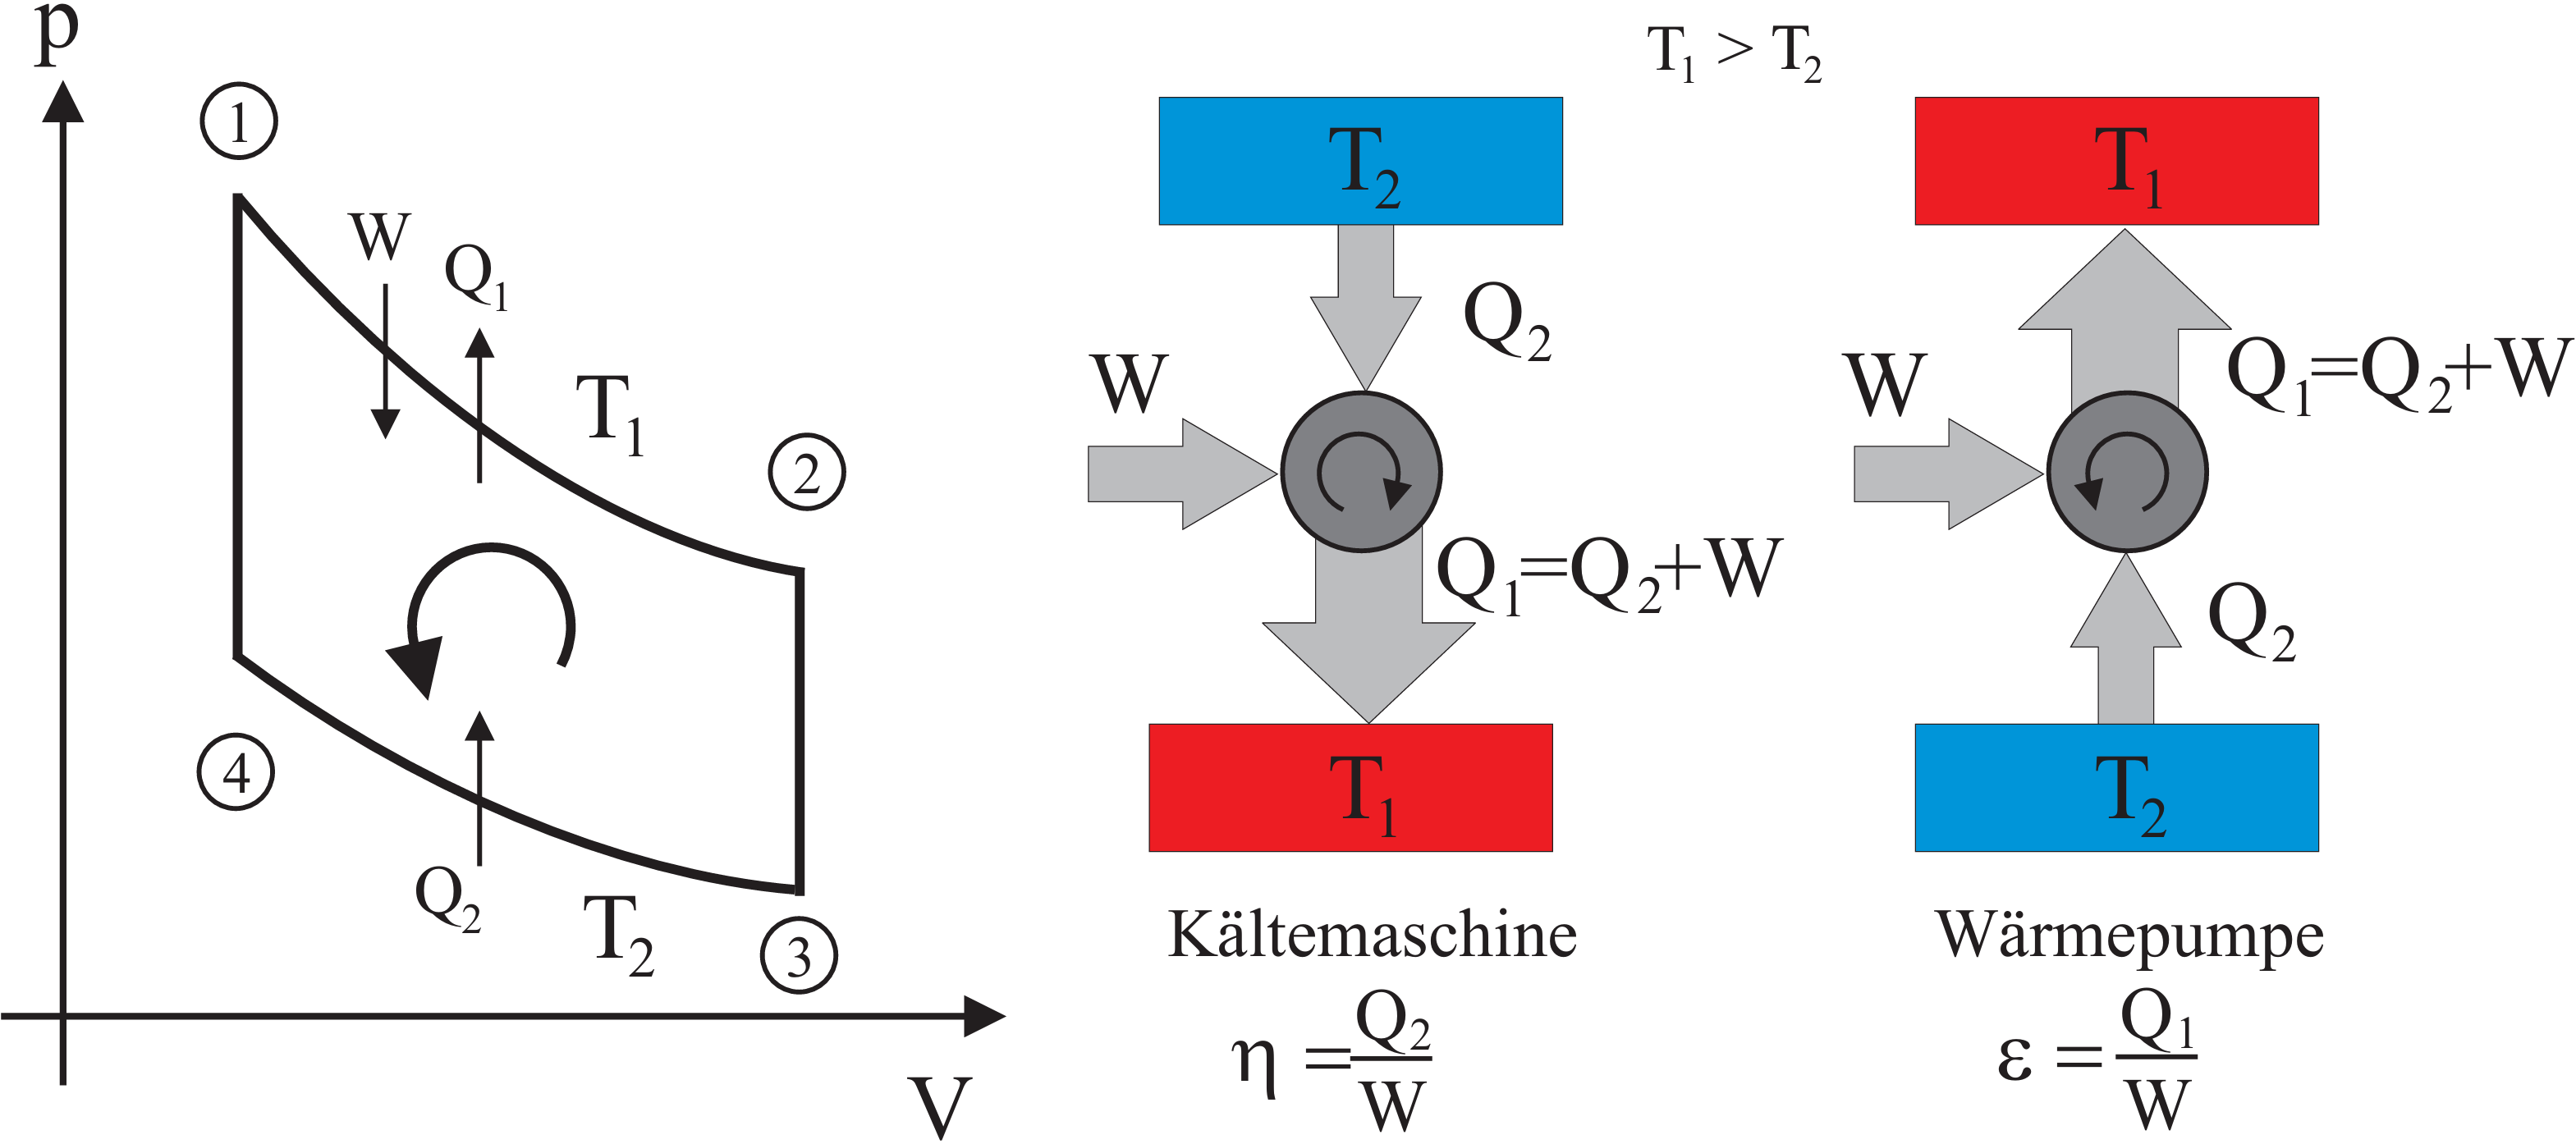
\includegraphics[width=.65\textwidth]{files/reverse_process_pv.png}
  \caption{Betrieb des Heißluftmotors als Kältemaschine oder Wärmepumpe}
  \label{fig:reverse_process_pv}
\end{figure}

Hierbei bestimmt die Antriebsrichtung des Schwungrades, ob der Motor als Kältemaschine oder Wärmepumpe fungiert. Dem oberen Bereich wird beim Betrieb als Kältemaschine die Wärmemenge $Q_2$ entzogen und die Wärmemenge $Q_1 = W + Q_2$ ab das Kühlsystem abgegeben. Umgekehrt wird beim Betrieb als Wärmepumpe dem Kühlwasser die Wärmemenge $Q_2$ entzogen und dem oberen Bereich die Wärmemenge $Q_1 = W + Q_2$ zugeführt. Hierbei beschreibt $W$ die durch den externen Antrieb zugeführte mechanische Arbeit. Für den Wirkungsgrad der Kältemaschine gilt
\begin{align}
  \eta = \frac{Q_2}{W} = \frac{T_2}{T_1 - T_2},
\end{align}
während die Effizienz der Wärmpumpe durch
\begin{align}
  \epsilon = \frac{Q_1}{W} = \frac{T_1}{T_1 - T_2},
\end{align}
genannt Leistungsziffer, angegeben ist.

Die bisher aufgezeigte mathematische Beschreibung, sowie die dargestellten pV-Digramme zeigen einen idealen Stirling-Prozesses auf, wie er in der Realität nicht möglich ist. Dieser ideale Stirling-Prozess ist technisch nicht realisierbar, da er eine diskontinuierliche Kolbenbewegung erfordern würde, was zu unruhigem Lauf und hohen Belastungen führt. Im Motor sind Arbeits- und Verdrängerkolben über die Kurbelwelle phasenverschoben gekoppelt, wodurch ein ruhiger Lauf, aber nur eine Annäherung an den idealen Prozess möglich sind. Durch Überlappungen der Zustandsänderungen entstehen Wirkungsgradverluste, was sich in einem abweichenden pV-Diagramm mit abgerundeten Isochoren, vlg. \abbref{fig:real_stirling_process}, zeigt.

\begin{figure}[H]
  \centering
  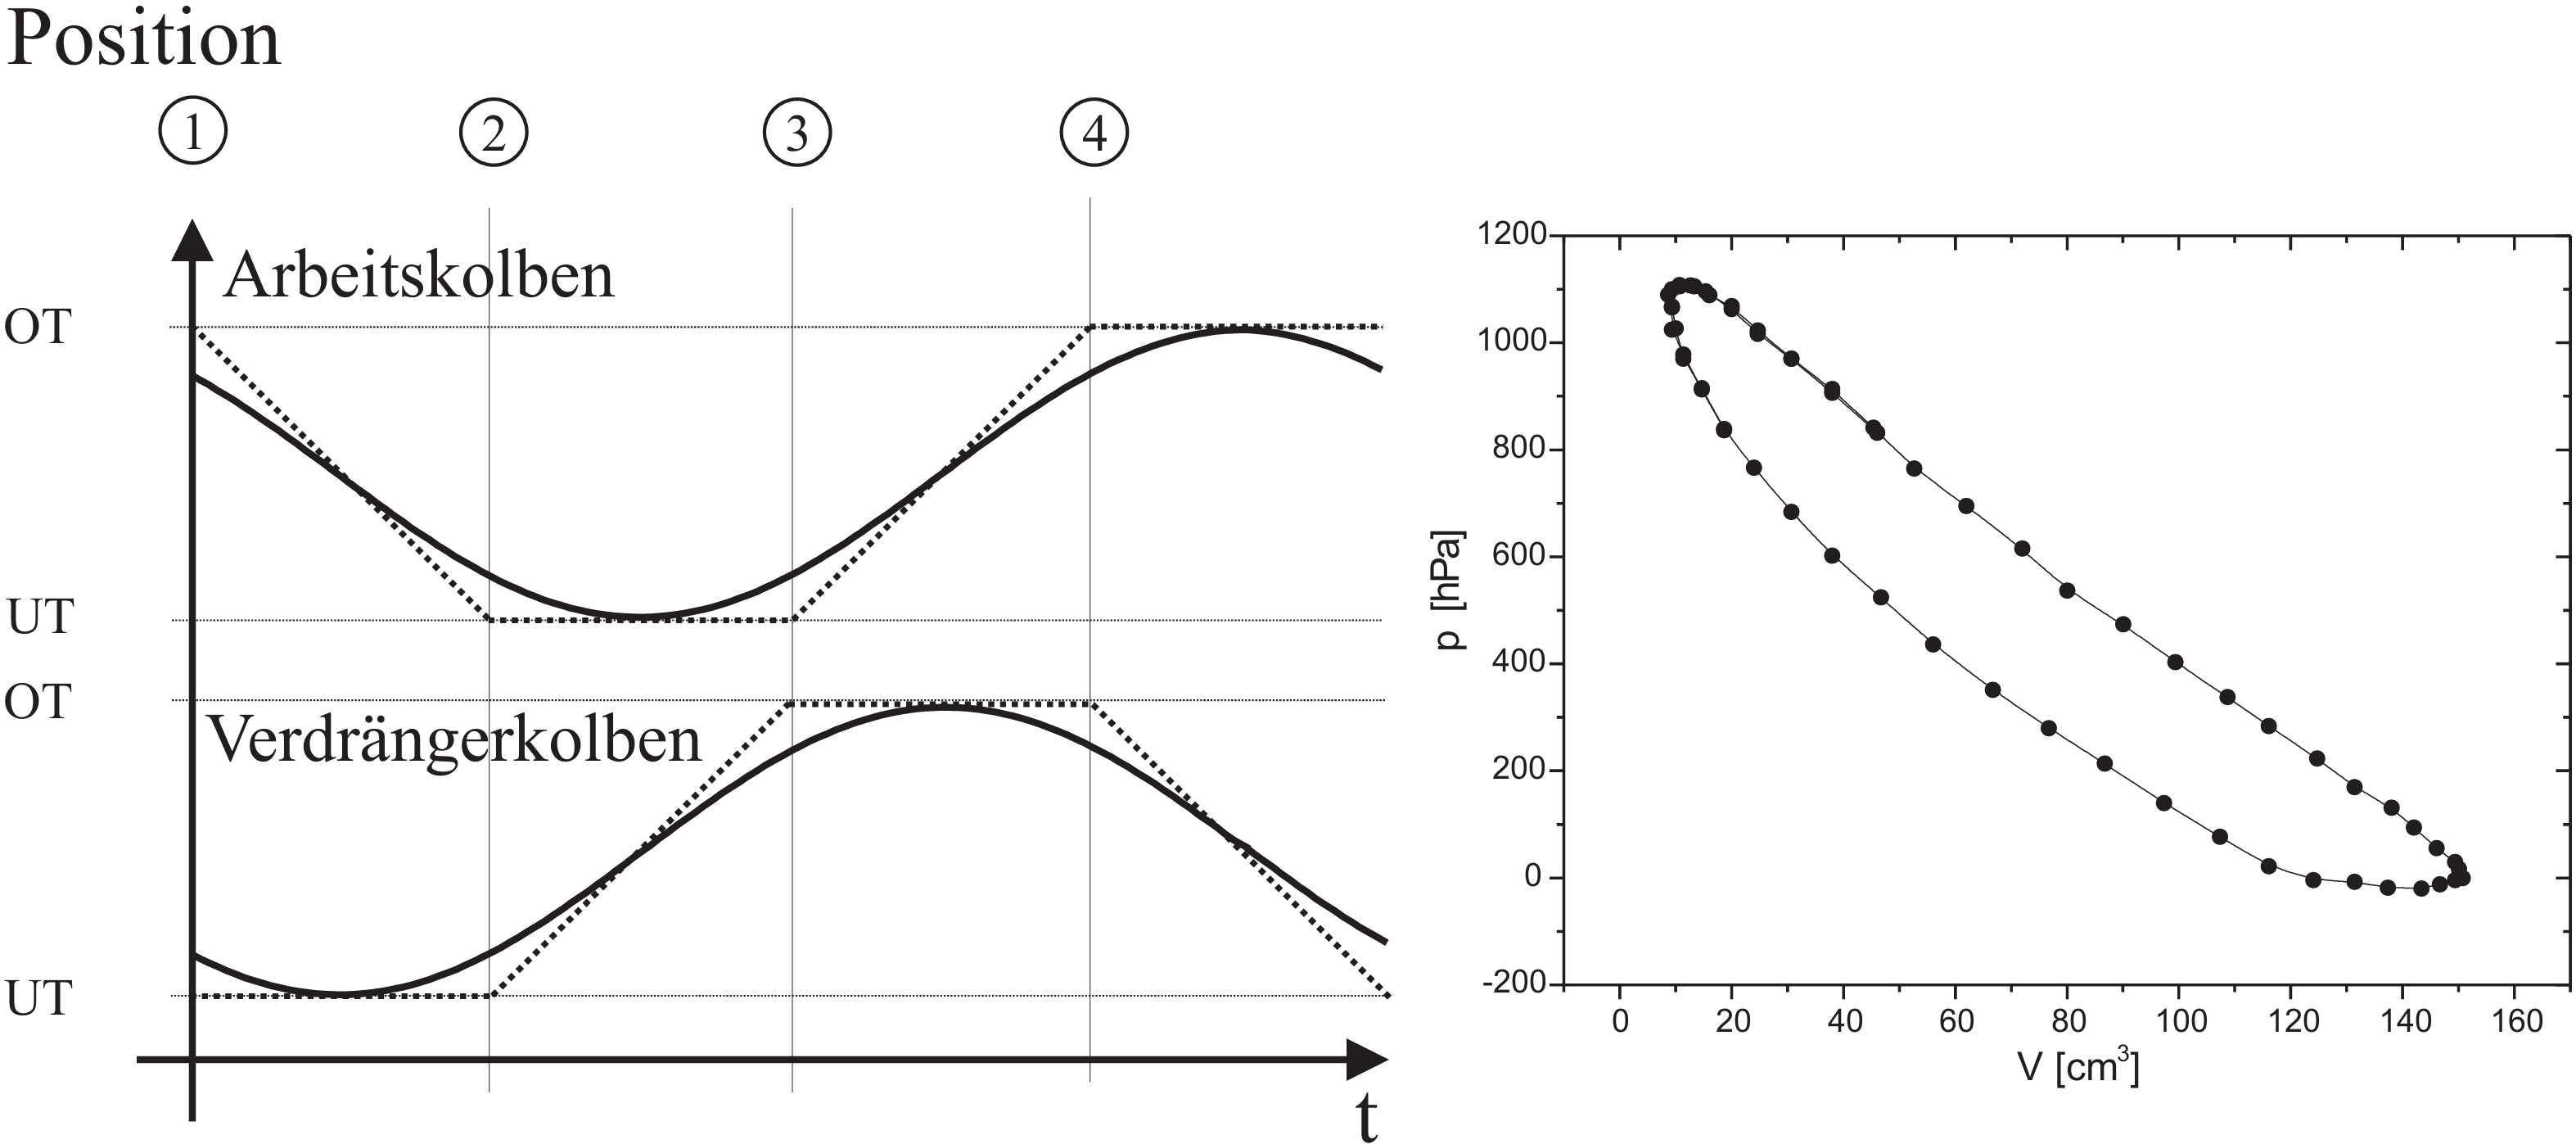
\includegraphics[width=.75\textwidth]{files/real_stirling_process.png}
  \caption{Der ideale Stirling-Prozess würde eine diskontinuierliche Kolbenbewegung voraussetzen. In Realität zeigt sich im pV-Diagramm eine Abrundung der Isochoren und damit verbunden Wirkungsgradverluste.}
  \label{fig:real_stirling_process}
\end{figure}
\newpage\noindent
\subsection{Versuchsdurchführung}

Der Versuch teilt sich in drei Blöcke auf, in welchen wir zunächst den umgekehrten Kreisprozess, sprich den Betrieb als Kältemaschine und Wärmepumpe, betrachten und im letzten Block den Betrieb als Wärmekraftmaschine.

\textbf{Betrieb als Kältemaschine und quantitative Bestimmung der Kälteleistung.} Wir betreiben den Motor als Kältemaschine, wodurch der obere Zylinderbereich zunächst abgekühlt wird. Gleichzeitig heizen wir den Bereich mit einer elektrischen Heizwendel auf, um in \glqq{}Summe\grqq{} wieder die Ausgangstemperatur zu erreichen. Wir messen in diesem Versuchsteil den Heizstrom $I_H$, die Heizspannung $U_H$, den Volumenfluss des Kühlwassers $\dot{V}$ und die Temperaturdifferenz $T_{ab} - T_{zu}$ des ab- und zufließenden Kühlwassers.

\textbf{Betrieb als Kältemaschine und Wärmepumpe.} In diesem Versuchsteil betreiben wir den Motor zunächst weiterhin als Kältemaschine. Anstatt der Heizwendel montieren wir nun ein Reagenzglas mit Wasser am oberen Teil des Zylinders. Im Wasser befindet sich ein Temperaturfühler, um die Temperatur des Wassers aufzuzeichnen. Wir betreiben die Kältemaschine bis die Temperatur des Wassers unter $0\si{\celsius}$ sinkt und dort einen konstanten erreicht. Dazu notieren wir uns den Motorstrom $I_M$, die Motorspannung $U_M$, Drehzahl $f$. Zusätzlich messen wir die Länge $t_f$ der Gefrierzeit des Wassers, welche an einem kurzen Plateau im Temperaturverlauf um die  $0\si{\celsius}$-Marke zu erkennen ist.


\textbf{Betrieb als Wärmekraftmaschine.} Wir bauen den externen Antrieb ab und installieren wieder die Heizwendel am oberen Zylinderbereich. Der Motor wird nun durch hinzugeben von Wärme durch die Heizwendel als Wärmekraftmaschine betrieben. Für die Leerlaufmessung lassen wir den Motor zunächst anlaufen und nehmen, sobald er eingelaufen ist, Heizstrom $I_H$, Heizspannung $U_H$, Durchflussmenge $\dot{V}$ des Kühlwassers, Temperaturdifferenz des $T_{ab} - T_{zu}$ ab- und zulaufenden Kühlwassers, Drehzahl $f$ des Schwungrades auf. Über die Software CASSY LAB zeichnen wir im diesem Versuchsteil zusätzlich die Fläche des pV-Diagrammes auf. Für den die weiteren Messungen bringen wir an der Motorwelle einen Bremszaum mit einem Federkraftmesser an, siehe \abbref{fig:motor_bremszaum}. Nachdem der Motor auch in diesem Aufbau eingelaufen ist stellen wir über den Bremszaum vier verschiedene Bremskräfte von $0.8\si{\newton}$ bis $0.2\si{\newton}$ ein und nehmen die Bremskraft $F$ vom Federkraftmesser, die Drehzahl $f$ des Schwungrades und die Fläche des pV-Diagrammes über die Software auf.

\begin{figure}[H]
  \centering
  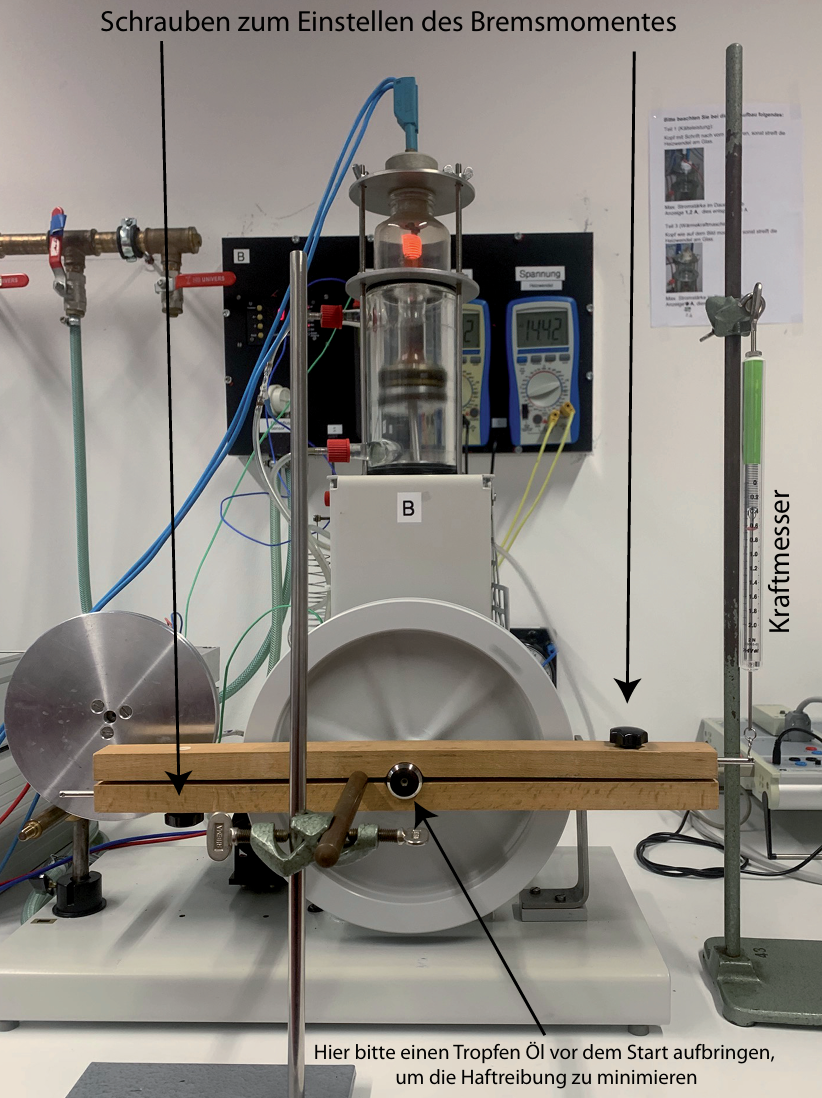
\includegraphics[width=.6\textwidth]{files/motor_bremszaum.png}
  \caption{Motoraufbau für Versuchteil 3 mit Bremszaum und Federkraftmesser}
  \label{fig:motor_bremszaum}
\end{figure}